% ===========================================================================
% MODELO DE RELATORIO  ·  ENE0046 Laboratorio de Eletronica  ·  2026/2
%
% Como usar
%   1. Preencha o bloco IDENTIFICACAO logo abaixo.
%   2. Deixe comentados os autores que nao existirem. Um autor fica centralizado,
%      dois dividem a linha, tres ocupam tercos.
%   3. Substitua o texto de cada secao pelo seu. As orientacoes que estao la
%      dizem o que se espera em cada uma.
%   4. Compile com pdflatex duas vezes, ou com latexmk -pdf.
%
% Estrutura
%   Roteiro 1 nao tem bancada: use so a subsecao 4.1 e a 5.1, e compare o calculo
%   analitico com a simulacao de projeto.
%   Roteiros 2 a 7 usam a estrutura inteira.
%
% O arquivo estilo-relatorio.tex deve estar na mesma pasta deste arquivo. A logo
% e as figuras ficam organizadas na subpasta imgs/, como no relatorio preenchido.
% ===========================================================================
\documentclass[11pt,a4paper]{article}
% !TeX root = modelo-relatorio.tex
% Formatacao do relatorio. Compile o modelo-relatorio.tex, nao este arquivo.
\usepackage[T1]{fontenc}
\usepackage[utf8]{inputenc}
\usepackage[brazil]{babel}
\usepackage[a4paper,top=1.6cm,bottom=1.8cm,left=2.1cm,right=2.1cm]{geometry}
\usepackage[default]{lato}
\usepackage{amsmath,amssymb}
\usepackage{siunitx}
\usepackage{graphicx}
\usepackage{booktabs,array,longtable,colortbl}
\usepackage{enumitem}
\usepackage{tcolorbox}
\usepackage{float}
\usepackage{xcolor}
\usepackage{tikz}
\usepackage{titlesec}
\usepackage{fancyhdr}
\usepackage{caption}
\usepackage{etoolbox}
\usepackage[colorlinks=true,linkcolor=azul,urlcolor=azul,citecolor=azul]{hyperref}
\tcbuselibrary{skins,breakable}

\definecolor{azul}{HTML}{0A4B8C}
\definecolor{azulclaro}{HTML}{E8F0F8}
\definecolor{verde}{HTML}{0B7A4B}
\definecolor{cinza}{HTML}{5B6672}
\definecolor{cinzaclaro}{HTML}{F4F6F8}
\definecolor{vinho}{HTML}{B04A4A}
\definecolor{vinhoclaro}{HTML}{FBF2F2}

\sisetup{output-decimal-marker={,}, per-mode=symbol}
\setlength{\parindent}{0pt}
\setlength{\parskip}{6pt plus 1pt}
\setlist{itemsep=3pt, topsep=4pt, parsep=0pt, leftmargin=1.3em}
\renewcommand{\arraystretch}{1.25}
\linespread{1.06}

% ---- secoes numeradas com marcador colorido -------------------------------
\titleformat{\section}[hang]
  {\Large\bfseries\color{azul}}
  {\raisebox{-1pt}{\tikz\node[fill=azul,text=white,rounded corners=2pt,
     inner sep=3pt,minimum width=20pt,align=center]{\bfseries\thesection};}}
  {10pt}{}
\titlespacing*{\section}{0pt}{16pt plus 3pt}{6pt}
\titleformat{\subsection}{\large\bfseries\color{cinza}}{\thesubsection}{8pt}{}
\titlespacing*{\subsection}{0pt}{11pt plus 2pt}{3pt}

% ---- legendas -------------------------------------------------------------
\captionsetup{font=small,labelfont={bf,color=azul},labelsep=period,skip=6pt}

% ---- identificacao --------------------------------------------------------
\newcommand{\autorA}{}\newcommand{\matA}{}
\newcommand{\autorB}{}\newcommand{\matB}{}
\newcommand{\autorC}{}\newcommand{\matC}{}
\newcommand{\autorum}[2]{\renewcommand{\autorA}{#1}\renewcommand{\matA}{#2}}
\newcommand{\autordois}[2]{\renewcommand{\autorB}{#1}\renewcommand{\matB}{#2}}
\newcommand{\autortres}[2]{\renewcommand{\autorC}{#1}\renewcommand{\matC}{#2}}

\newcommand{\disciplina}{ENE0046 · Laboratório de Eletrônica}
\newcommand{\semestre}{2026/2}
\newcommand{\turma}{}
\newcommand{\roteironum}{}
\newcommand{\roteirotema}{}
\newcommand{\aturma}[1]{\renewcommand{\turma}{#1}}
\newcommand{\roteiro}[2]{\renewcommand{\roteironum}{#1}\renewcommand{\roteirotema}{#2}}

\newcommand{\umautor}[2]{%
  \begin{minipage}[t]{\dimexpr\linewidth-4pt\relax}\centering
    \parbox[t][30pt][t]{\linewidth}{\centering
      {\fontsize{10.5}{12.5}\selectfont #1}}\\[-2pt]
    {\color{cinza}\fontsize{9}{11}\selectfont\texttt{#2}}
  \end{minipage}}

\newcounter{nautores}
\newcommand{\blocoautores}{%
  \setcounter{nautores}{0}%
  \ifdefempty{\autorA}{}{\stepcounter{nautores}}%
  \ifdefempty{\autorB}{}{\stepcounter{nautores}}%
  \ifdefempty{\autorC}{}{\stepcounter{nautores}}%
  \ifnum\value{nautores}=0
    \begin{center}\color{vinho}\bfseries
      Preencha ao menos um autor no preâmbulo do arquivo.
    \end{center}
  \else
    \begin{center}
    \ifcase\value{nautores}\or
      % --- um autor: ocupa o centro
      \begin{minipage}{0.5\textwidth}\umautor{\autorA}{\matA}\end{minipage}%
    \or
      % --- dois autores: metades
      \begin{minipage}{0.42\textwidth}\umautor{\autorA}{\matA}\end{minipage}\hspace{0.04\textwidth}%
      \begin{minipage}{0.42\textwidth}\umautor{\autorB}{\matB}\end{minipage}%
    \or
      % --- tres autores: tercos
      \begin{minipage}{0.31\textwidth}\umautor{\autorA}{\matA}\end{minipage}\hspace{0.015\textwidth}%
      \begin{minipage}{0.31\textwidth}\umautor{\autorB}{\matB}\end{minipage}\hspace{0.015\textwidth}%
      \begin{minipage}{0.31\textwidth}\umautor{\autorC}{\matC}\end{minipage}%
    \fi
    \end{center}
  \fi}

% ---- cabecalho do relatorio -----------------------------------------------
\newcommand{\capa}{%
\begin{tcolorbox}[colback=azul,colframe=azul,boxrule=0pt,arc=4pt,
  left=16pt,right=16pt,top=13pt,bottom=13pt]
\color{white}
\begin{minipage}{0.76\textwidth}
  {\fontsize{9}{11}\selectfont\textbf{\MakeUppercase{\disciplina{} · \semestre{}}}}\\[6pt]
  {\fontsize{22}{25}\selectfont\bfseries Relatório do Roteiro \roteironum}\\[3pt]
  {\fontsize{12.5}{15}\selectfont \roteirotema}
\end{minipage}\hfill
\begin{minipage}{0.2\textwidth}\raggedleft
  \colorbox{white}{\hspace{2pt}\raisebox{-2pt}{\includegraphics[height=30pt]{imgs/logo-unb.png}}\hspace{2pt}}
\end{minipage}
\end{tcolorbox}
\vspace{10pt}
\blocoautores
\ifdefempty{\turma}{}{%
  \begin{center}{\color{cinza}\fontsize{9}{11}\selectfont Turma \turma}\end{center}}
\vspace{4pt}
{\color{azulclaro}\hrule height 2pt}
\vspace{2pt}}

% ---- caixas auxiliares ----------------------------------------------------
\newtcolorbox{formula}{colback=azulclaro,colframe=azul,boxrule=0.8pt,arc=3pt,
  left=12pt,right=12pt,top=9pt,bottom=9pt}
\newtcolorbox{nota}[1]{colback=cinzaclaro,colframe=cinza,boxrule=0.8pt,arc=3pt,
  left=10pt,right=10pt,top=7pt,bottom=7pt,
  title={\textbf{#1}},fonttitle=\small\bfseries,coltitle=white,colbacktitle=cinza}
\newenvironment{resumo}
  {\vspace{6pt}\begin{center}\begin{minipage}{0.92\textwidth}
   \begin{tcolorbox}[colback=cinzaclaro,colframe=cinzaclaro,boxrule=0pt,arc=3pt,
     left=14pt,right=14pt,top=10pt,bottom=10pt,
     borderline west={2.5pt}{0pt}{azul}]
   {\color{azul}\fontsize{8}{10}\selectfont\textbf{RESUMO}}\\[4pt]
   \small}
  {\end{tcolorbox}\end{minipage}\end{center}\vspace{2pt}}

\newtcolorbox{espec}{colback=azulclaro,colframe=azul,boxrule=0.8pt,arc=3pt,
  left=12pt,right=12pt,top=9pt,bottom=9pt,
  title={\textbf{Especificação da matrícula}},fonttitle=\bfseries,
  coltitle=white,colbacktitle=azul}

\newtcolorbox{especbancada}{colback=azulclaro,colframe=azul,boxrule=0.8pt,arc=3pt,
  left=12pt,right=12pt,top=9pt,bottom=9pt,
  title={\textbf{Especificação da Equipe}},fonttitle=\bfseries,
  coltitle=white,colbacktitle=azul}

% ---- rodape ---------------------------------------------------------------
\pagestyle{fancy}\fancyhf{}
\renewcommand{\headrulewidth}{0pt}
\renewcommand{\footrulewidth}{0.4pt}
\fancyfoot[L]{\color{cinza}\fontsize{8}{10}\selectfont \disciplina{} · \semestre{} · Roteiro \roteironum}
\fancyfoot[R]{\color{cinza}\fontsize{8}{10}\selectfont \thepage}

\newlist{referencias}{itemize}{1}
\setlist[referencias]{label={}, leftmargin=1.1em, itemindent=-1.1em,
                     itemsep=3pt, topsep=2pt, parsep=0pt}

\newcommand{\mat}[1]{\texttt{\textbf{#1}}}


% --------------------------- IDENTIFICACAO ---------------------------------
\roteiro{1}{Simulação de Circuitos: Introdução ao LTspice}
\aturma{03}

\autorum{Lurian Correia Lima}{22/2005395} 
\autordois{Guilherme Cardoso Oliveira da Silva Júnior}{23/1038626}
\autortres{Daniel Campos Silva}{23/1036775}
% ---------------------------------------------------------------------------

\begin{document}
\capa

\begin{resumo}
% Escreva este parágrafo por último, com 100 a 150 palavras. Diga o que você projetou, sob
% qual especificação, o que simulou ou mediu, o principal resultado numérico e a que
% conclusão chegou. Quem ler só este parágrafo deve saber o que você fez e o que encontrou.
\end{resumo}

\section{Introdução}

% Comece pelo problema, e não pelo circuito. Que necessidade de engenharia deu origem a esta
% topologia, onde você a encontraria em um equipamento real e o que aconteceria sem ela. Duas
% ou três referências ajudam aqui.

% Depois estreite o foco: que aspecto você vai investigar, sob quais condições, e por que
% vale a pena verificá-lo. Se o roteiro impõe alguma restrição de projeto que parece
% arbitrária, aproveite para explicar a razão dela.

% No último parágrafo, diga qual é o objetivo deste relatório e como o texto está
% organizado, seção a seção.

\section{Fundamentação teórica}

% Deduza as expressões que você vai usar mais adiante, partindo das leis de circuito.
% Numere as equações que forem retomadas no restante do texto.

% \begin{equation}
% H(j\omega) = \frac{1}{1+j\omega RC}
% \label{eq:exemplo}
% \end{equation}

% Toda grandeza que aparecer nos resultados precisa ter sido apresentada aqui. Explique o que
% cada termo significa fisicamente, não apenas o que a letra representa. Registre as hipóteses
% que você está assumindo, como linearidade ou idealidade dos componentes: se alguma delas
% não se sustentar no experimento, você vai retomá-la na discussão.

% Se o circuito tiver regimes de funcionamento distintos, apresente cada um e diga o que os
% separa.

\section{Especificação e projeto}

\begin{espec}

\textbf{Matrícula \mat{23/1038626}.} Considerando os nove dígitos na forma ABCDEFGHI, com o dígito I não nulo,

\begin{equation}
    A=2,\; B=3,\; C=1,\; D=0,\; E=3,\; F=8,\; G=6,\; H=2,\; I=6
\end{equation}

A partir desses valores, as especificações individuais exigidas pelo roteiro são:

\begin{itemize}
    \item \textbf{Fonte:} \\
    Senoide de 60 Hz com $AB = 23\text{ V}$ de pico a pico. Logo, a amplitude é $V_p = 11{,}5\text{ V}$.

    \vspace{0.3cm}
    
    \item \textbf{Regulação (Zener):} \\
    O diodo Zener da série BZX84C cuja tensão nominal mais se aproxima de $\frac{V_p}{\sqrt{2}} = \frac{11{,}5}{\sqrt{2}} \approx 8{,}13\text{ V}$. Na lista do LTspice, o valor mais próximo é de \textbf{8,2 V}.
    
    \vspace{0.3cm}
    
    \item \textbf{Carga (Corrente):} \\
    Corrente $I_L = I \times 100\,\mu\text{A} = 6 \times 100\,\mu\text{A} = 600\,\mu\text{A} = 0{,}6\text{ mA}$ na tensão regulada de $8{,}2\text{ V}$.
\end{itemize}

\end{espec}

Os componentes da série comercial E12 selecionados para atender a cada especificação, bem como os desvios e dimensionamentos, são detalhados a seguir:

\begin{itemize}

    \item \textbf{Carga ($R_L$):} 
    A resistência de carga necessária para drenar a corrente especificada na tensão regulada é calculada por $R_L = \frac{V_Z}{I_L} = \frac{8{,}2}{0{,}6 \times 10^{-3}} \approx 13{,}67\,\mathrm{k}\Omega$. O valor comercial E12 adotado nas simulações é $R_L = 15\,\mathrm{k}\Omega$. O uso desse resistor na tensão nominal de $8{,}2\text{ V}$ drena efetivamente $I_{L,\text{real}} = \frac{8{,}2}{15\,\mathrm{k}\Omega} \approx 0{,}547\text{ mA}$. Esse $R_L$ é mantido constante em todas as seções de simulação.

    \item \textbf{Capacitor de Filtro ($C_1$):}
    O dimensionamento do capacitor para um \textit{ripple} máximo ($V_r$) de $1{,}5\text{ V}$ de pico a pico num retificador de meia onda ($f = 60\text{ Hz}$) é determinado pela Equação 1 do roteiro:
    \[
    C_1 \approx \frac{I_L}{f \cdot V_r} = \frac{0{,}6 \times 10^{-3}}{60 \times 1{,}5} \approx 6{,}67\,\mu\text{F}
    \]
    Para garantir um ripple próximo ao especificado, arredonda-se para o valor E12 imediatamente superior, resultando na escolha de $C_1 = 6{,}8\,\mu\text{F}$. O capacitor dez vezes maior testado na simulação \texttt{item\_3.asc} é de $68\,\mu\text{F}$.

    \item \textbf{Resistor Série do Regulador ($R_S$):}
    Para calcular $R_S$, utiliza-se a tensão mínima na saída do filtro ($V_{min}$) na onda completa. Projetando o \textit{ripple} com $f = 120\text{ Hz}$:
    \[
    V_r \approx \frac{0{,}6 \times 10^{-3}}{120 \times 6{,}8 \times 10^{-6}} \approx 0{,}735\text{ V}
    \]
    A tensão de pico na onda completa (considerando a queda de dois diodos de aproximadamente $0{,}7\text{ V}$ cada) é $V_{p,\text{carga}} \approx 11{,}5 - 1{,}4 = 10{,}1\text{ V}$. Logo, $V_{min} \approx 10{,}1 - 0{,}735 = 9{,}365\text{ V}$.
    O valor de $R_S$ para assegurar que a corrente no Zener não fique inferior a $I_{Z,min} = 1\text{ mA}$ no vale do ripple é dado pela Equação 2:
    \[
    R_S = \frac{V_{min} - V_Z}{I_L + I_{Z,min}} = \frac{9{,}365 - 8{,}2}{0{,}6 \times 10^{-3} + 1 \times 10^{-3}} = \frac{1{,}165}{1{,}6 \times 10^{-3}} \approx 728\,\Omega
    \]
    Arredondando para o valor E12 mais próximo que mantém a regulação, adotou-se $R_S = 820\,\Omega$. 
    
    Verificando a potência máxima no Zener com a carga retirada ($I_L = 0$) e na crista do sinal ($V_{max} \approx 10{,}1\text{ V}$):
    \[
    I_{Z,max} = \frac{V_{max} - V_Z}{R_S} = \frac{10{,}1 - 8{,}2}{820} \approx 2{,}32\text{ mA}
    \]
    \[
    P_{Z,max} = V_Z \times I_{Z,max} = 8{,}2 \times 2{,}32\text{ mA} \approx 19{,}0\text{ mW}
    \]
    Este valor está extremamente abaixo do limite de $250\text{ mW}$ do BZX84C, tornando o projeto seguro.

\end{itemize}

A tabela abaixo resume os parâmetros teóricos e os adotados:

\begin{center}
\renewcommand{\arraystretch}{1.2}
\begin{tabular}{@{}lrrr@{}}
\toprule
\textbf{Grandeza} & \textbf{Teórico} & \textbf{Adotado (E12)} & \textbf{Desvio} \\
\midrule
Amplitude da Fonte ($V_p$) & $11{,}50\text{ V}$ & $11{,}50\text{ V}$ & $0{,}00\%$ \\
Tensão de Regulação ($V_Z$) & $8{,}13\text{ V}$ & $8{,}20\text{ V}$ & $0{,}86\%$ \\
Corrente da Carga ($I_L$ em $8{,}2\text{ V}$) & $0{,}60\text{ mA}$ & $0{,}547\text{ mA}$ & $-8{,}83\%$ \\
Resistor de Carga ($R_L$) & $13{,}67\text{ k}\Omega$ & $15\text{ k}\Omega$ & $9{,}73\%$ \\
Capacitor de Filtro ($C_1$) & $6{,}67\,\mu\text{F}$ & $6{,}8\,\mu\text{F}$ & $1{,}95\%$ \\
Resistor do Zener ($R_S$) & $728\,\Omega$ & $820\,\Omega$ & $12{,}64\%$ \\
\bottomrule
\end{tabular}
\end{center}

% Transcreva os parâmetros que a sua matrícula determina, mostrando a conta a partir dos
% dígitos.

% \begin{espec}
% Matrícula \mat{00/0000000}. \\
% Preencha aqui os parâmetros calculados a partir dos dígitos, conforme o roteiro.
% \end{espec}

% Leve cada parâmetro até o valor de componente, deixando visível a expressão que você
% inverteu para chegar lá. Depois escolha o valor na série comercial e calcule o quanto essa
% escolha afasta você do valor ideal. A tabela abaixo organiza isso, e é ela que depois
% permite separar o que veio do projeto do que veio da montagem.

% \begin{center}
% \begin{tabular}{@{}lrrr@{}}
% \toprule
% \textbf{Grandeza} & \textbf{Teórico} & \textbf{Adotado} & \textbf{Desvio} \\
% \midrule
% & & & \\
% \bottomrule
% \end{tabular}
% \end{center}

% Se mais de uma combinação atender à especificação, diga por que escolheu esta, mostrando
% que as outras ficavam mais distantes.

\section{Metodologia}

% Conte o que você fez e com quais parâmetros, de modo que um colega consiga repetir sem
% precisar perguntar nada. Explique as escolhas que não são evidentes: por que essa faixa de
% varredura, por que esse passo de integração, por que esse intervalo de gravação.

% Inclua a figura do esquemático, com legenda que descreva o que ela mostra, e cite-a no
% texto, como na Figura~\ref{fig:exemplo}. Se uma figura não for mencionada em nenhum
% parágrafo, ela provavelmente não precisa estar aqui.

\subsection{Simulação de projeto, uma por integrante}

% Cada integrante recebeu uma especificação diferente da própria matrícula, e portanto chegou
% a um dimensionamento diferente. Traga aqui \textbf{uma simulação por integrante}, cada uma
% com os componentes que aquela pessoa projetou. São elas que mostram se cada projeto cumpre
% o que foi pedido.

\subsubsection{Guilherme Cardoso Oliveira da Silva Júnior (23/1038626)}

\textbf{Configuração e Simulação dos Circuitos}

Para comprovar que o projeto atende às especificações apresentadas na Seção 3 (referentes à retificação, filtragem e regulação de tensão), os seis circuitos foram desenhados e simulados no LTspice, conforme a Figura~\ref{fig:circs_guilherme}. Em todas as análises, adotou-se a diretiva de regime transitório (\texttt{.tran 0 100m}) para abranger o tempo correspondente a seis períodos da rede elétrica de 60 Hz. Os esquemáticos foram configurados da seguinte forma:

\begin{itemize}
    \item \textbf{Retificador de meia onda (Fig.~\ref{fig:circs_guilherme}a):} A fonte de entrada foi configurada com uma senoide de 60 Hz e 11,5 V de amplitude (\texttt{SINE(0 11.5 60)}), alimentando a carga $R_L$ de 15 k$\Omega$ através de um único diodo 1N4007. 
    
    \item \textbf{Meia onda com filtro (Fig.~\ref{fig:circs_guilherme}b):} Adicionou-se o capacitor eletrolítico de filtro $C_1$ de 6,8 $\mu$F em paralelo com a carga. O objetivo é sustentar a tensão entre os semiciclos de condução e permitir a leitura do \textit{ripple} gerado.

    \item \textbf{Meia onda com filtro 10x maior (Fig.~\ref{fig:circs_guilherme}c):} O capacitor $C_1$ foi substituído por um de 68 $\mu$F. Essa simulação visa observar a atenuação teórica do \textit{ripple} e o impacto no pico de corrente exigido do diodo durante o seu tempo de condução.
    
    \item \textbf{Ponte retificadora sem filtro (Fig.~\ref{fig:circs_guilherme}d):} Montou-se a topologia de onda completa com quatro diodos 1N4007. A referência do circuito (terra) foi posicionada no nó inferior da carga, deixando a fonte senoidal flutuante para reproduzir o comportamento correto da diferença de potencial.

    \item \textbf{Ponte com filtro (Fig.~\ref{fig:circs_guilherme}e):} O capacitor de 6,8 $\mu$F foi reintroduzido na saída da ponte retificadora. Esta etapa permite comparar o \textit{ripple} em 120 Hz com o resultado obtido na retificação de meia onda para o mesmo valor de capacitância.

    \item \textbf{Regulação com Zener (Fig.~\ref{fig:circs_guilherme}f):} Acrescentou-se o resistor de limitação $R_S$ de 820 $\Omega$ e o diodo Zener \texttt{BZX84C8V2L} de 8,2 V em paralelo com a carga. A configuração demonstra a estabilização final da tensão contínua e a supressão do \textit{ripple} remanescente.
\end{itemize}

\begin{figure}[H]
\centering
\begin{minipage}{0.48\linewidth}
    \centering
    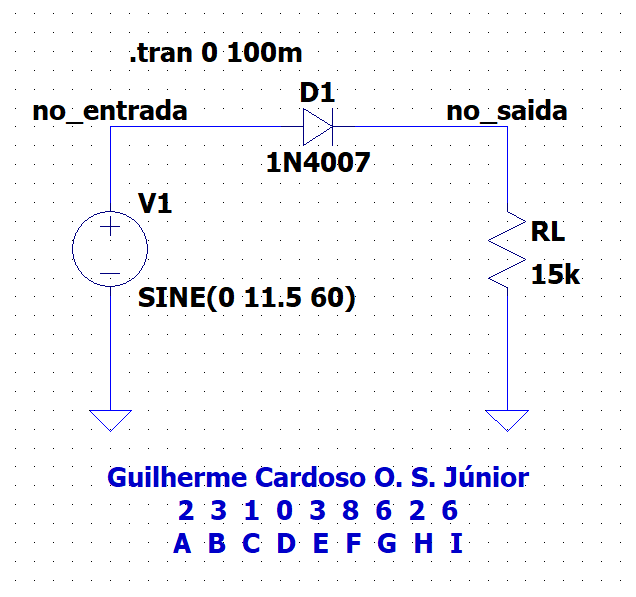
\includegraphics[width=\linewidth]{imgs/cardoso/simulação/item_1_diagrama.png}
    \vspace{2pt}
    {\small (a) Retificador de meia onda}
\end{minipage}\hfill
\begin{minipage}{0.48\linewidth}
    \centering
    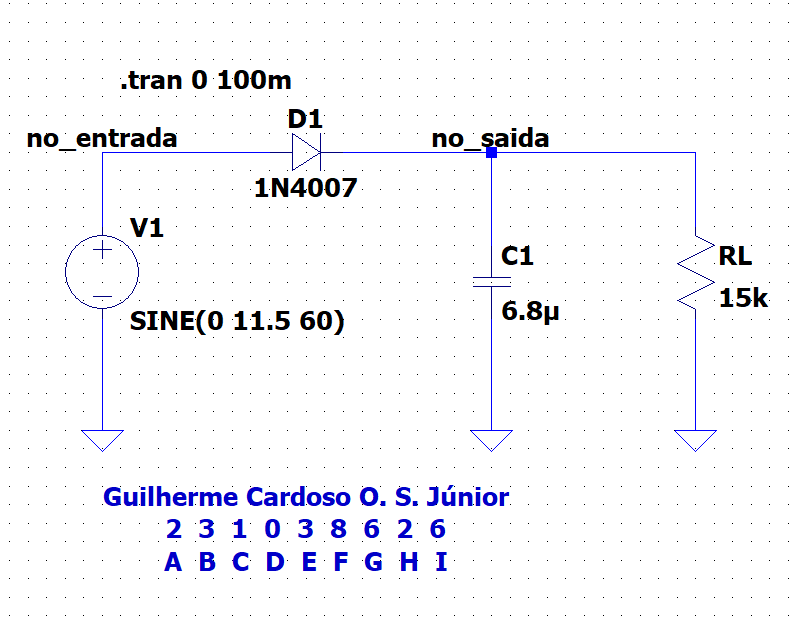
\includegraphics[width=\linewidth]{imgs/cardoso/simulação/item_2_diagrama.png}
    \vspace{2pt}
    {\small (b) Meia onda com filtro de 6,8 $\mu$F}
\end{minipage}

\vspace{12pt}

\begin{minipage}{0.48\linewidth}
    \centering
    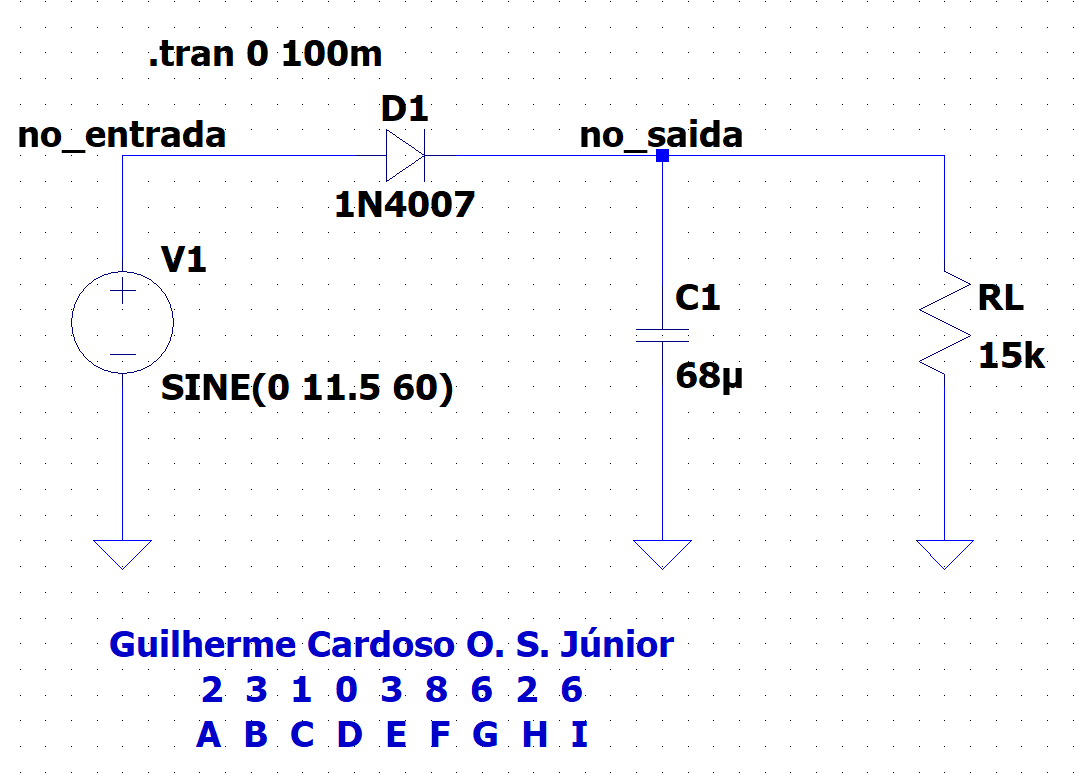
\includegraphics[width=\linewidth]{imgs/cardoso/simulação/item_3_diagrama.png}
    \vspace{2pt}
    {\small (c) Meia onda com filtro 10x maior (68 $\mu$F)}
\end{minipage}\hfill
\begin{minipage}{0.48\linewidth}
    \centering
    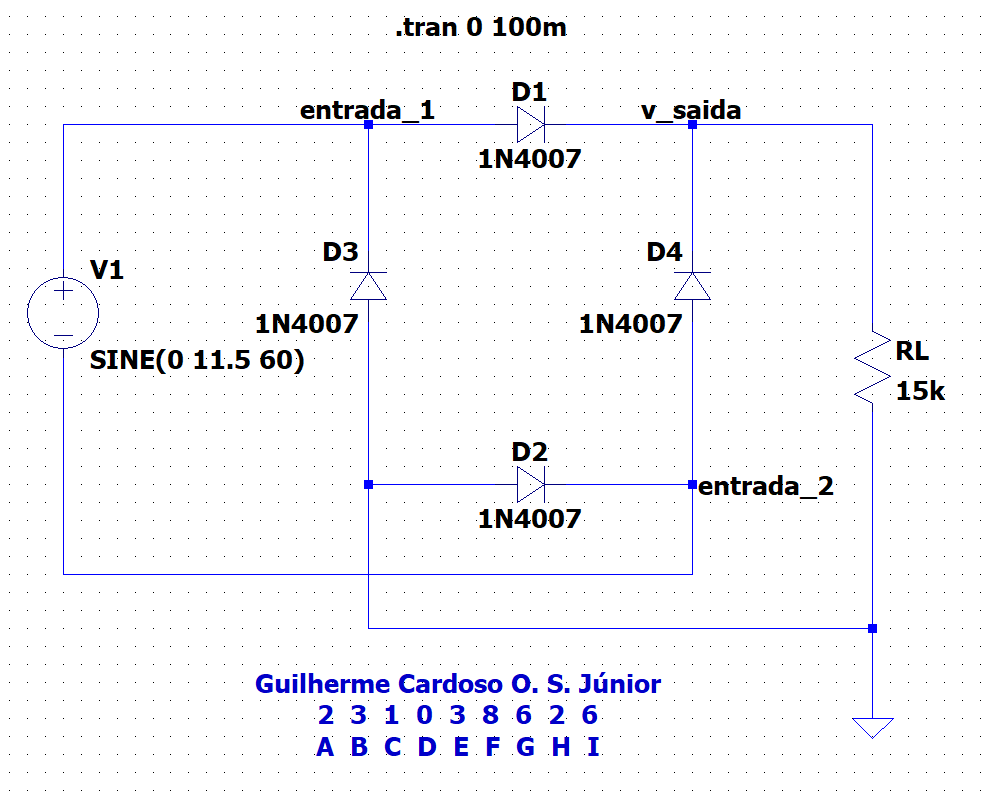
\includegraphics[width=\linewidth]{imgs/cardoso/simulação/item_4_diagrama.png}
    \vspace{2pt}
    {\small (d) Ponte retificadora sem filtro}
\end{minipage}

\vspace{12pt}

\begin{minipage}{0.48\linewidth}
    \centering
    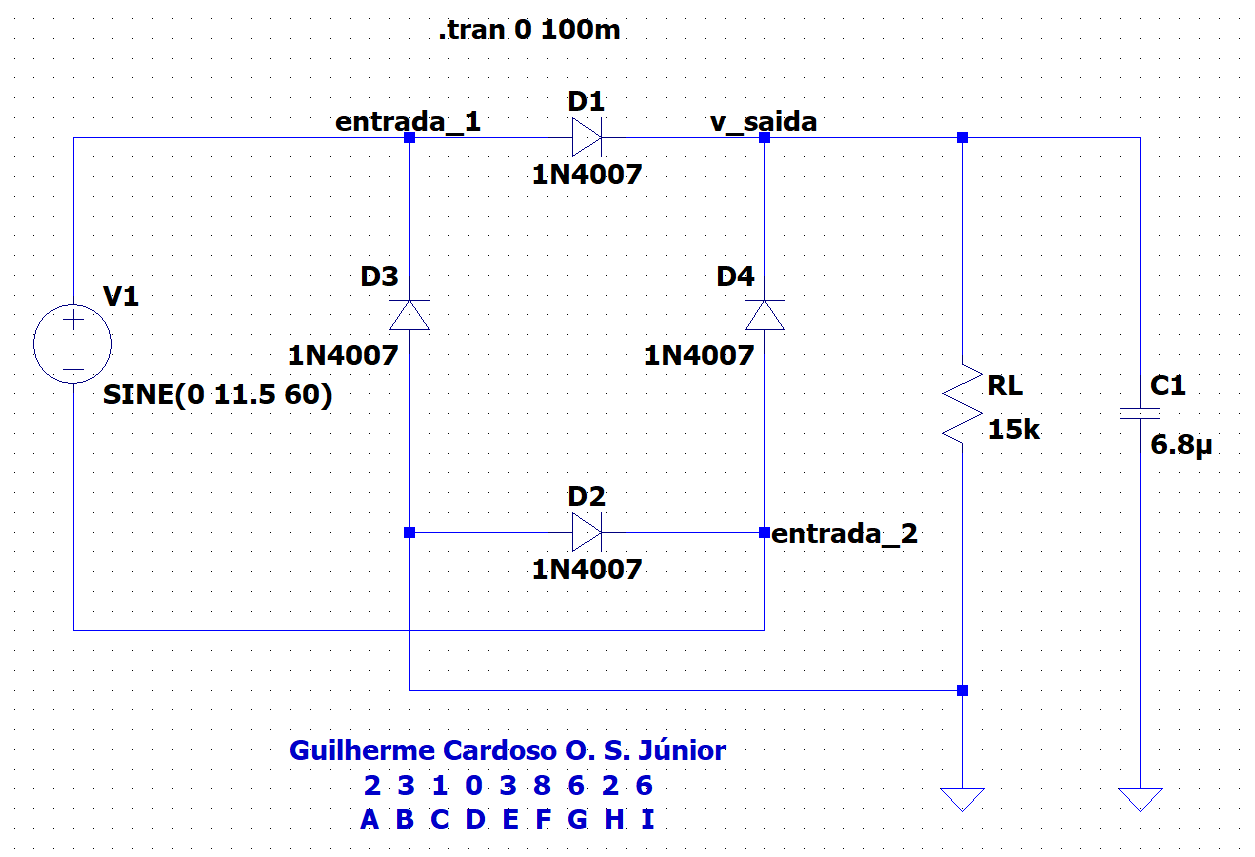
\includegraphics[width=\linewidth]{imgs/cardoso/simulação/item_5_diagrama.png}
    \vspace{2pt}
    {\small (e) Ponte retificadora com filtro}
\end{minipage}\hfill
\begin{minipage}{0.48\linewidth}
    \centering
    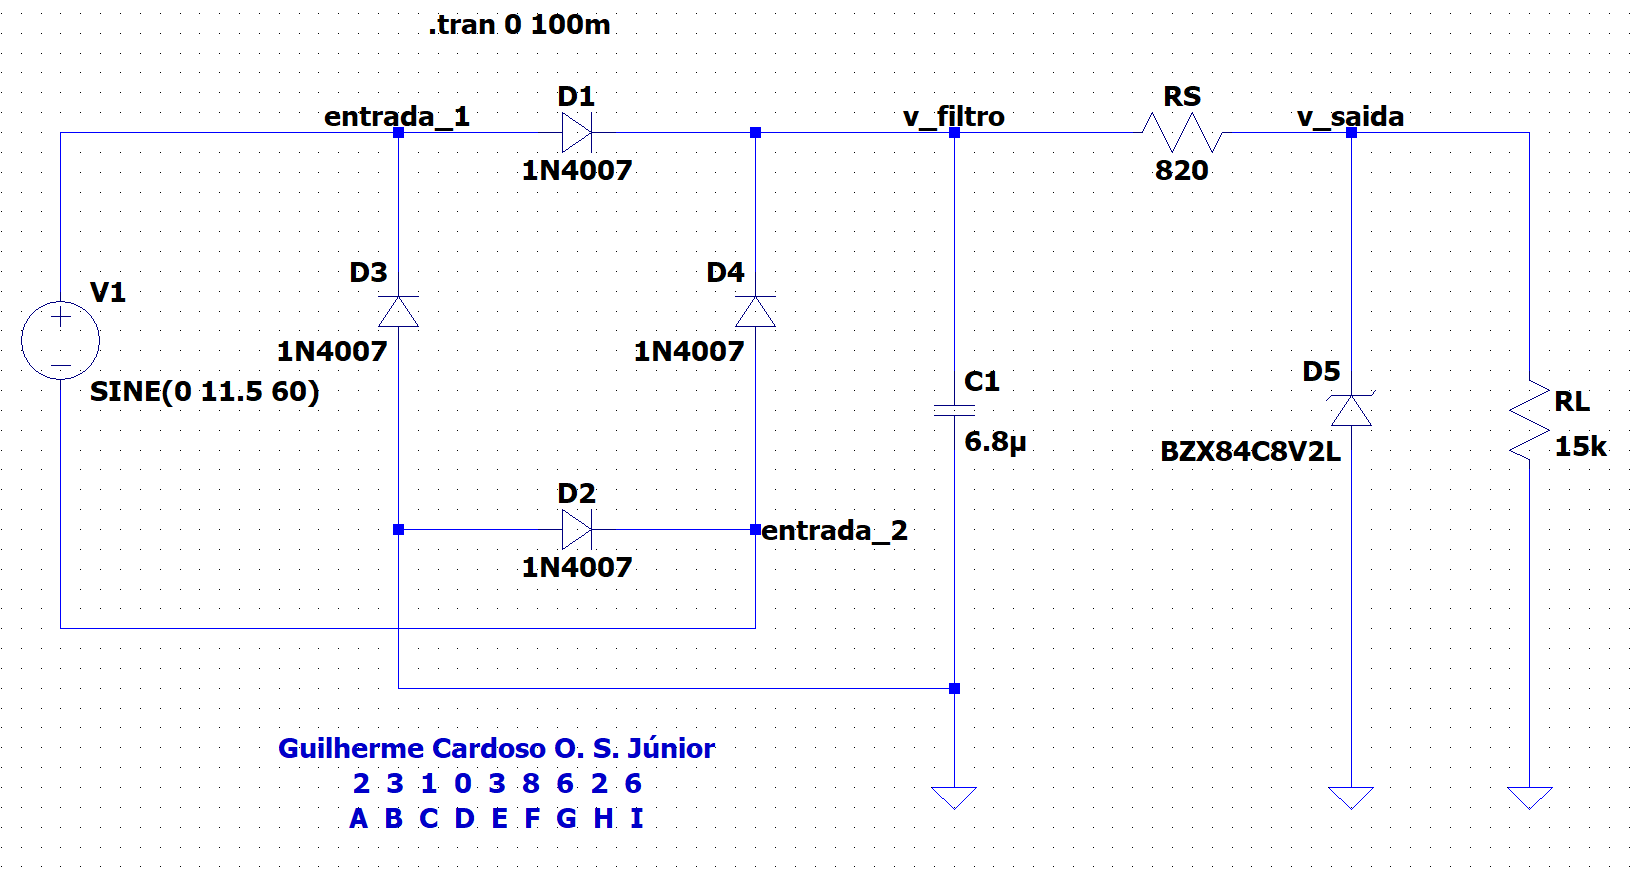
\includegraphics[width=\linewidth]{imgs/cardoso/simulação/item_6_diagrama.png}
    \vspace{2pt}
    {\small (f) Regulação com Zener (Cadeia completa)}
\end{minipage}

\caption{Esquemáticos projetados para a matrícula 23/1038626 contendo os componentes da série E12 e a diretiva de simulação de regime transitório aplicada para cada etapa da fonte linear.}
\label{fig:circs_guilherme}
\end{figure}

\subsection{Montagem em bancada}

% A equipe monta um circuito só. Diga \textbf{de quem} é a especificação que vocês montaram e
% por que escolheram essa. Informe os valores \textbf{medidos} de cada componente que vocês
% usaram, e não os valores nominais impressos no corpo da peça, porque a diferença entre os
% dois explica boa parte do que vocês vão observar.

\subsection{Simulação da montagem}

% Refaça a simulação usando os valores medidos dos componentes que estavam na bancada. Ela
% não substitui a simulação de projeto: é a comparação entre as duas que separa o efeito da
% tolerância dos componentes do restante.

\begin{nota}{Três comparações, três causas diferentes}
% Ao longo do relatório vocês vão confrontar três pares de resultados. Cada um responde a uma
% pergunta distinta, e vale mantê-los separados na hora de discutir.

% \smallskip
% \textbf{Cálculo analítico contra simulação de projeto.} A conta está certa? Se aqui houver
% diferença, procure na álgebra ou no esquemático.

% \smallskip
% \textbf{Simulação de projeto contra simulação da montagem.} Quanto custou a tolerância dos
% componentes? A diferença aqui é a distância entre o valor nominal e o valor real da peça
% que vocês pegaram.

% \smallskip
% \textbf{Simulação da montagem contra medição.} O modelo descreve o circuito real? Diferença
% aqui aponta algo que o modelo não representa, como a resistência série do indutor, a
% impedância da ponta de prova ou a banda do instrumento.
\end{nota}

% \begin{figure}[htb]
% \centering
% % \includegraphics[width=0.8\linewidth]{arquivo.png}
% \fbox{\parbox[c][3.2cm][c]{0.8\linewidth}{\centering\color{cinza}
%   substitua por \texttt{\textbackslash includegraphics}}}
% \caption{Legenda descritiva. Diga o que a figura mostra e o que nela é relevante, e não
% apenas o nome do circuito.}
% \label{fig:exemplo}
% \end{figure}

\section{Resultados}

% Apresente o que vocês obtiveram, em tabela sempre que houver mais de dois números. Use o
% número de algarismos significativos que a medição sustenta, e não todos os que o programa
% imprime. Para cada leitura de bancada, informe o instrumento e a incerteza.

% Guarde a interpretação para a seção seguinte: aqui vocês mostram o que encontraram.

\subsection{Projeto de cada integrante}

% Uma tabela por integrante, ou uma tabela única com uma coluna por integrante, confrontando
% o valor analítico e o simulado para cada grandeza pedida no roteiro.

\subsubsection{Guilherme Cardoso Oliveira da Silva Júnior (23/1038626)}

A Tabela~\ref{tab:resultados_cardoso} apresenta os parâmetros projetados analiticamente a partir dos componentes da série E12, confrontando-os com os resultados medidos nas simulações de regime transitório (\texttt{.tran}) no LTspice.

\begin{table}[H]
    \centering
    \caption{Resultados simulados dos estágios da fonte de alimentação (Matrícula 23/1038626).}
    \label{tab:resultados_cardoso}
    \renewcommand{\arraystretch}{1.2}
    \begin{tabular}{@{}lrrr@{}}
    \toprule
    \textbf{Grandeza} & \textbf{Analítico (E12)} & \textbf{Simulado} & \textbf{Erro (\%)} \\
    \midrule    
    Tensão de Pico na Carga (Meia Onda) & $10{,}80\text{ V}$ & $10{,}92\text{ V}$ & $1{,}11\%$ \\
    Tensão Média na Carga (Meia Onda) & $3{,}48\text{ V}$ & $3{,}39\text{ V}$ & $-2{,}58\%$ \\
    Ripple Meia Onda ($C=6{,}8\text{ }\mu\text{F}$) & $1{,}34\text{ V}$ & $1{,}49\text{ V}$ & $11{,}19\%$ \\
    Tensão de Pico na Carga (Onda Completa) & $10{,}10\text{ V}$ & $10{,}35\text{ V}$ & $2{,}47\%$ \\
    Tensão Média na Carga (Onda Completa) & $6{,}59\text{ V}$ & $6{,}26\text{ V}$ & $-5{,}00\%$ \\
    Ripple Onda Completa ($C=6{,}8\text{ }\mu\text{F}$) & $0{,}67\text{ V}$ & $0{,}68\text{ V}$ & $1{,}49\%$ \\
    Tensão Regulada Média (Zener) & $8{,}20\text{ V}$ & $8{,}18\text{ V}$ & $-0{,}24\%$ \\
    \bottomrule
    \multicolumn{4}{l}{\footnotesize O valor analítico do ripple utilizou $I_L \approx 0{,}547\text{ mA}$ (carga real E12 de $15\text{ k}\Omega$).}
    \end{tabular}
\end{table}

\paragraph{Análise da Retificação de Meia Onda (Itens 1, 2 e 3):}
No circuito sem filtro, a tensão de pico atingiu $10{,}92\text{ V}$. A diferença em relação ao pico da fonte ($11{,}5\text{ V}$) é de $0{,}58\text{ V}$, o que comprova analiticamente a queda de tensão direta de um único diodo 1N4007 em condução. O valor médio medido ($3{,}39\text{ V}$) esteve coerente com o cálculo teórico para meia onda ($V_p/\pi \approx 3{,}48\text{ V}$).
Ao inserir o capacitor de $6{,}8\text{ }\mu\text{F}$, o \textit{ripple} simulado foi de $1{,}49\text{ V}$, valor próximo aos $1{,}34\text{ V}$ previstos pela Equação 1. A simulação revelou que a largura do pulso de recarga do capacitor dura apenas $\Delta t = 1{,}62\text{ ms}$. Em um período de $60\text{ Hz}$ ($16{,}67\text{ ms}$), o diodo conduz por apenas $9{,}7\%$ do tempo. Para compensar essa estreita janela, o pico de corrente no diodo atingiu $13{,}9\text{ mA}$, um valor mais de $25$ vezes superior à corrente contínua exigida pela carga ($0{,}547\text{ mA}$).
Quando o capacitor foi aumentado em 10 vezes ($68\text{ }\mu\text{F}$), o \textit{ripple} caiu para quase um décimo do valor original ($0{,}165\text{ V}$), atestando a relação inversamente proporcional da Equação 1. Contudo, essa capacitância maior reduziu ainda mais a fração de condução, elevando drasticamente o pico de corrente no diodo para $29{,}3\text{ mA}$.

\paragraph{Análise da Ponte Retificadora (Itens 4 e 5):}
Na topologia de onda completa sem filtro, o pico na carga mediu $10{,}35\text{ V}$. A atenuação em relação à fonte foi de $1{,}15\text{ V}$, o dobro da observada na meia onda, o que é justificado analiticamente pelo fato de a corrente atravessar sempre dois diodos em série a cada semiciclo. O valor médio medido ($6{,}26\text{ V}$) aproximou-se da teoria ($2V_p/\pi \approx 6{,}59\text{ V}$).
Ao conectar o filtro de $6{,}8\text{ }\mu\text{F}$, o \textit{ripple} simulado reduziu para $0{,}68\text{ V}$. Esse valor representa essencialmente a metade da oscilação vista na meia onda ($1{,}49\text{ V}$), confirmando que dobrar a frequência de recarga (de $60\text{ Hz}$ para $120\text{ Hz}$) atenua proporcionalmente a descarga, estabelecendo uma tensão mínima na saída do filtro ($V_{min}$) de $9{,}62\text{ V}$.

\paragraph{Análise da Regulação com Zener (Item 6):}
O estágio regulador introduziu o resistor $R_S$ de $820\,\Omega$ em série. A maior drenagem de corrente alterou o \textit{ripple} na saída do filtro capacitivo para $1{,}43\text{ V}$. Em contrapartida, na carga em paralelo com o diodo Zener, o \textit{ripple} remanescente foi de apenas $0{,}14\text{ V}$. A razão entre eles indica que o Zener atenuou a oscilação em cerca de $10$ vezes ($\approx 20\text{ dB}$).
Analiticamente, a regulação é mantida pois o Zener nunca entra em corte. No vale do \textit{ripple}, a simulação apontou que ainda circula $I_{Z,min} = 0{,}31\text{ mA}$. No pico, a corrente sobe para $I_{Z,max} = 1{,}88\text{ mA}$. Retirando-se a carga, a corrente máxima convergiria para $I_Z = (V_{max\_filtro} - V_Z)/R_S \approx (10{,}24 - 8{,}2)/820 \approx 2{,}48\text{ mA}$. A potência dissipada máxima ($8{,}2\text{ V} \times 2{,}48\text{ mA} \approx 20{,}3\text{ mW}$) respeita com larga folga os limites de $250\text{ mW}$ (BZX84C) e $500\text{ mW}$ (1N754), atestando a robustez térmica do projeto.

\begin{figure}[H]
    \centering
    \begin{minipage}[b]{0.48\linewidth}
        \centering
        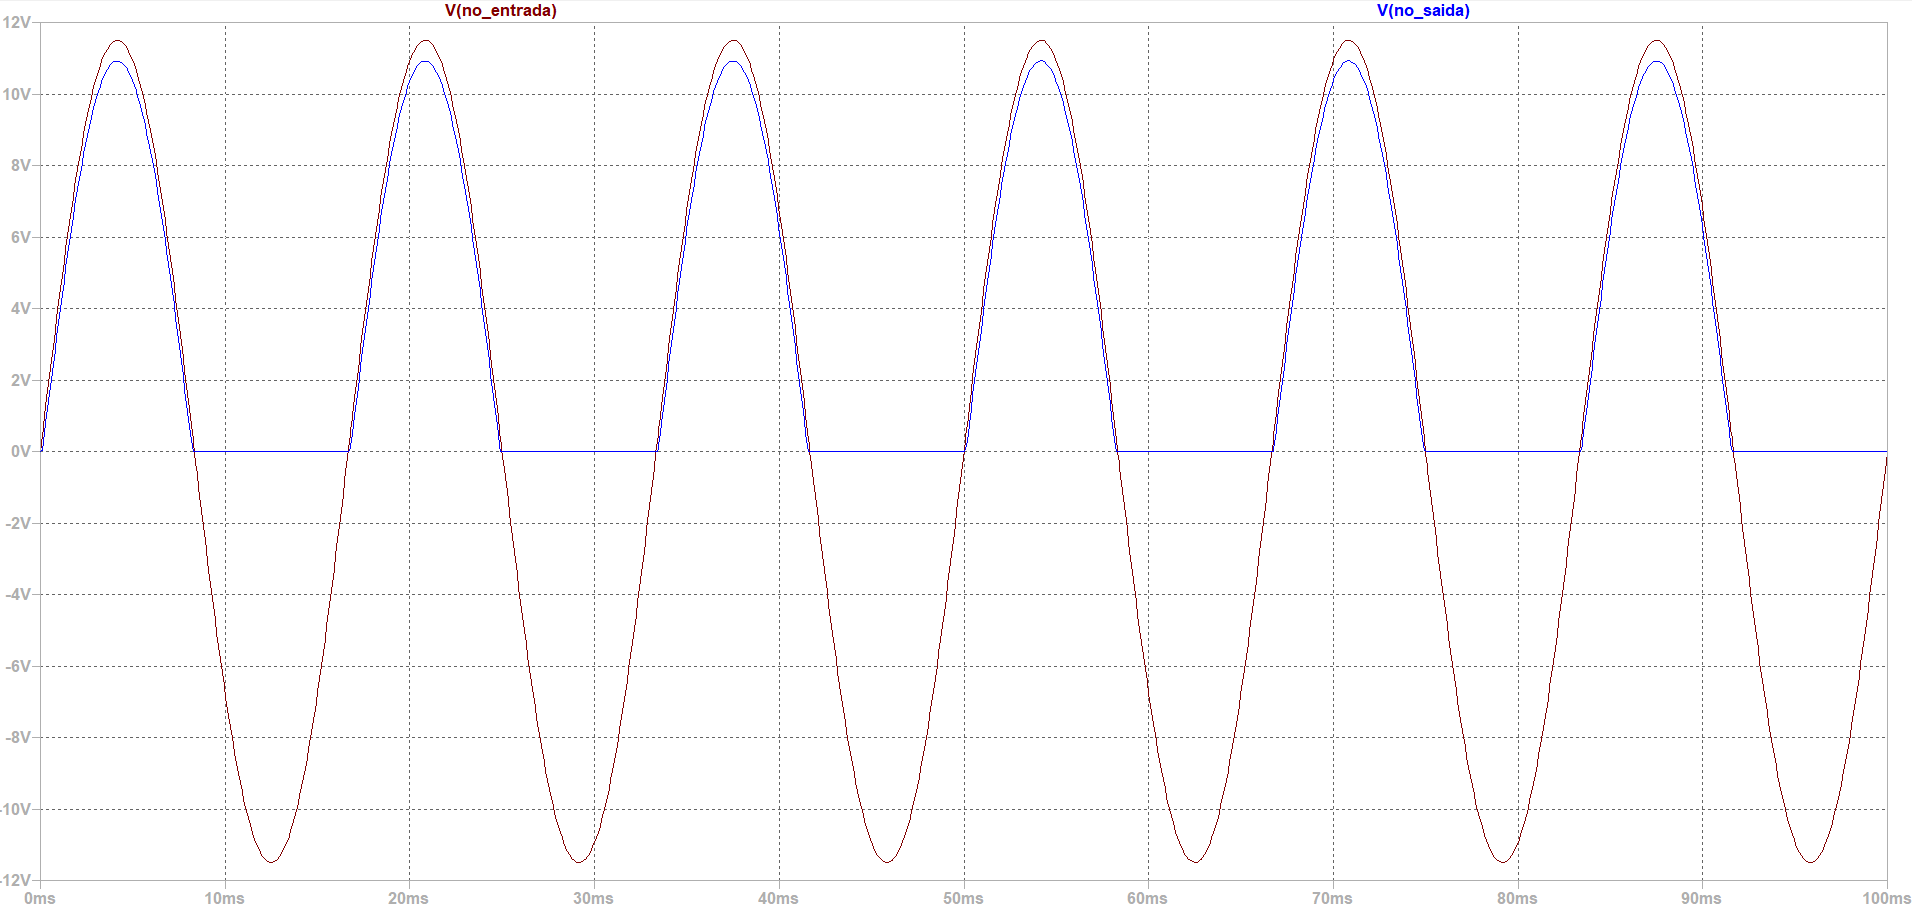
\includegraphics[width=\linewidth]{imgs/cardoso/resultados/simulacao_item_1_exp5.png}
        \vspace{2pt}
        {\small (a) Tensão: Meia onda sem filtro.}
    \end{minipage}%
    \hfill
    \begin{minipage}[b]{0.48\linewidth}
        \centering
        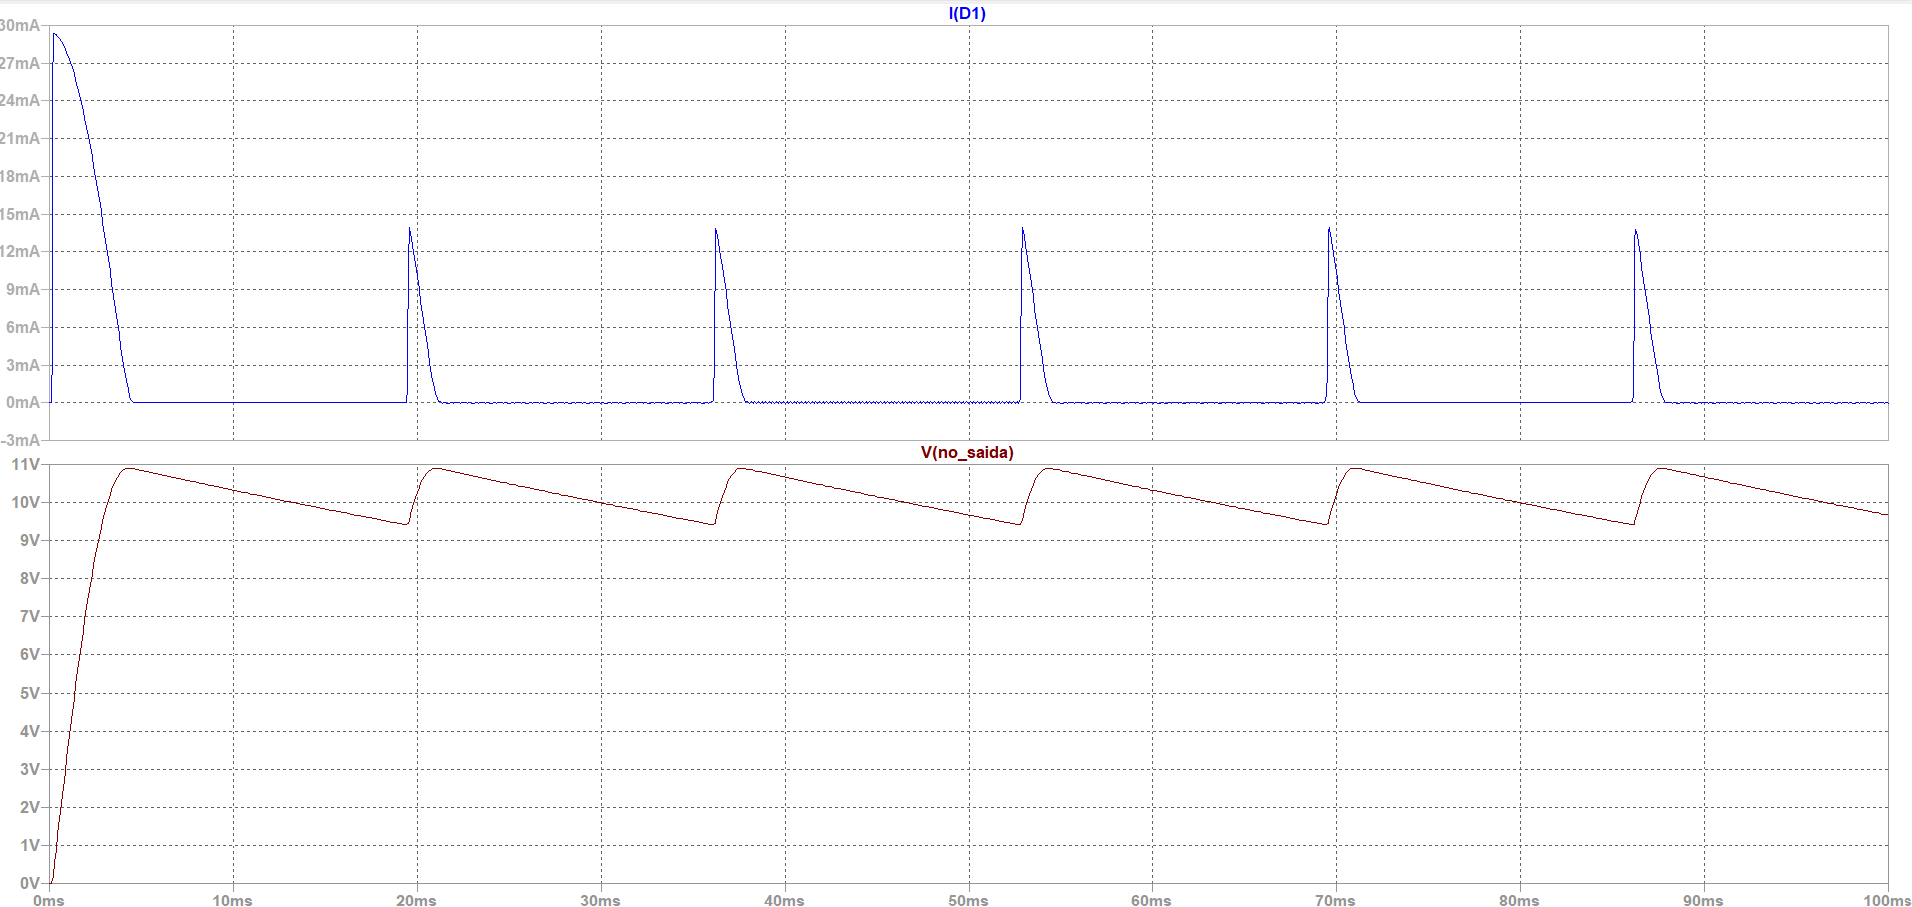
\includegraphics[width=\linewidth]{imgs/cardoso/resultados/simulacao_item_2_exp5.png}
        \vspace{2pt}
        {\small (b) Tensão e Corrente: Filtro de $6{,}8\text{ }\mu\text{F}$.}
    \end{minipage}

    \vspace{12pt}

    \begin{minipage}[b]{0.48\linewidth}
        \centering
        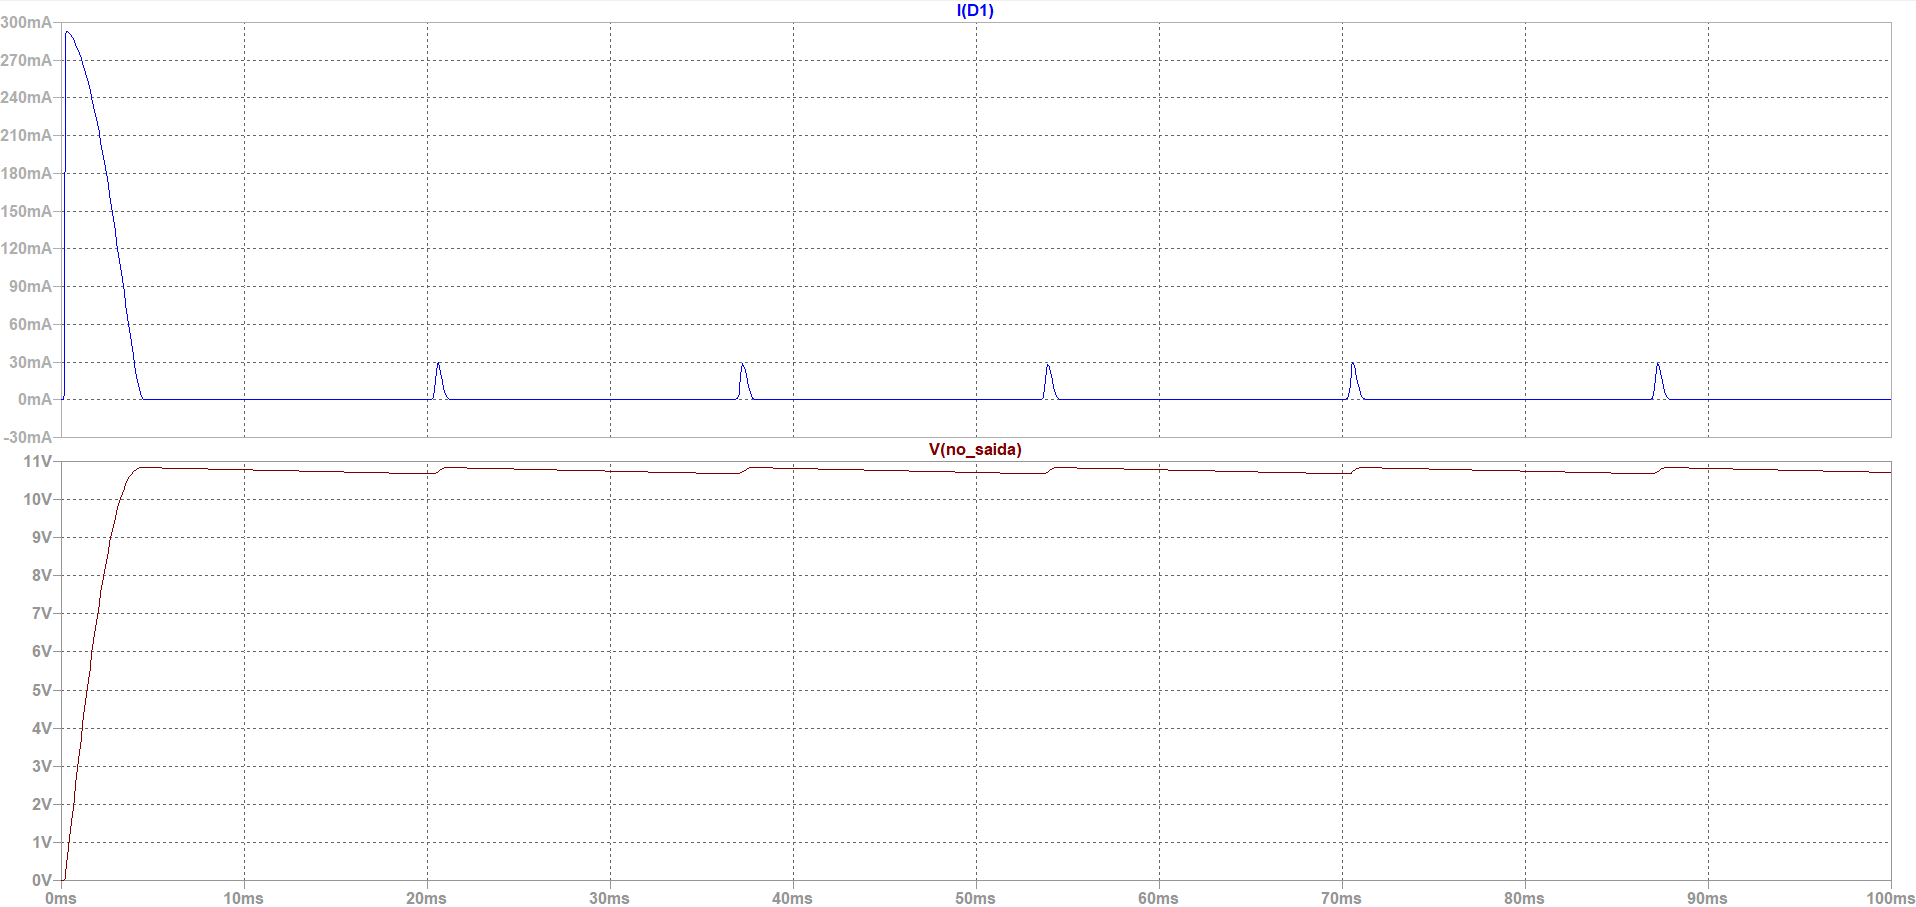
\includegraphics[width=\linewidth]{imgs/cardoso/resultados/simulacao_item_3_exp5.png}
        \vspace{2pt}
        {\small (c) Tensão e Corrente: Filtro de $68\text{ }\mu\text{F}$.}
    \end{minipage}
    \hfill
    \begin{minipage}[b]{0.48\linewidth}
        \centering
        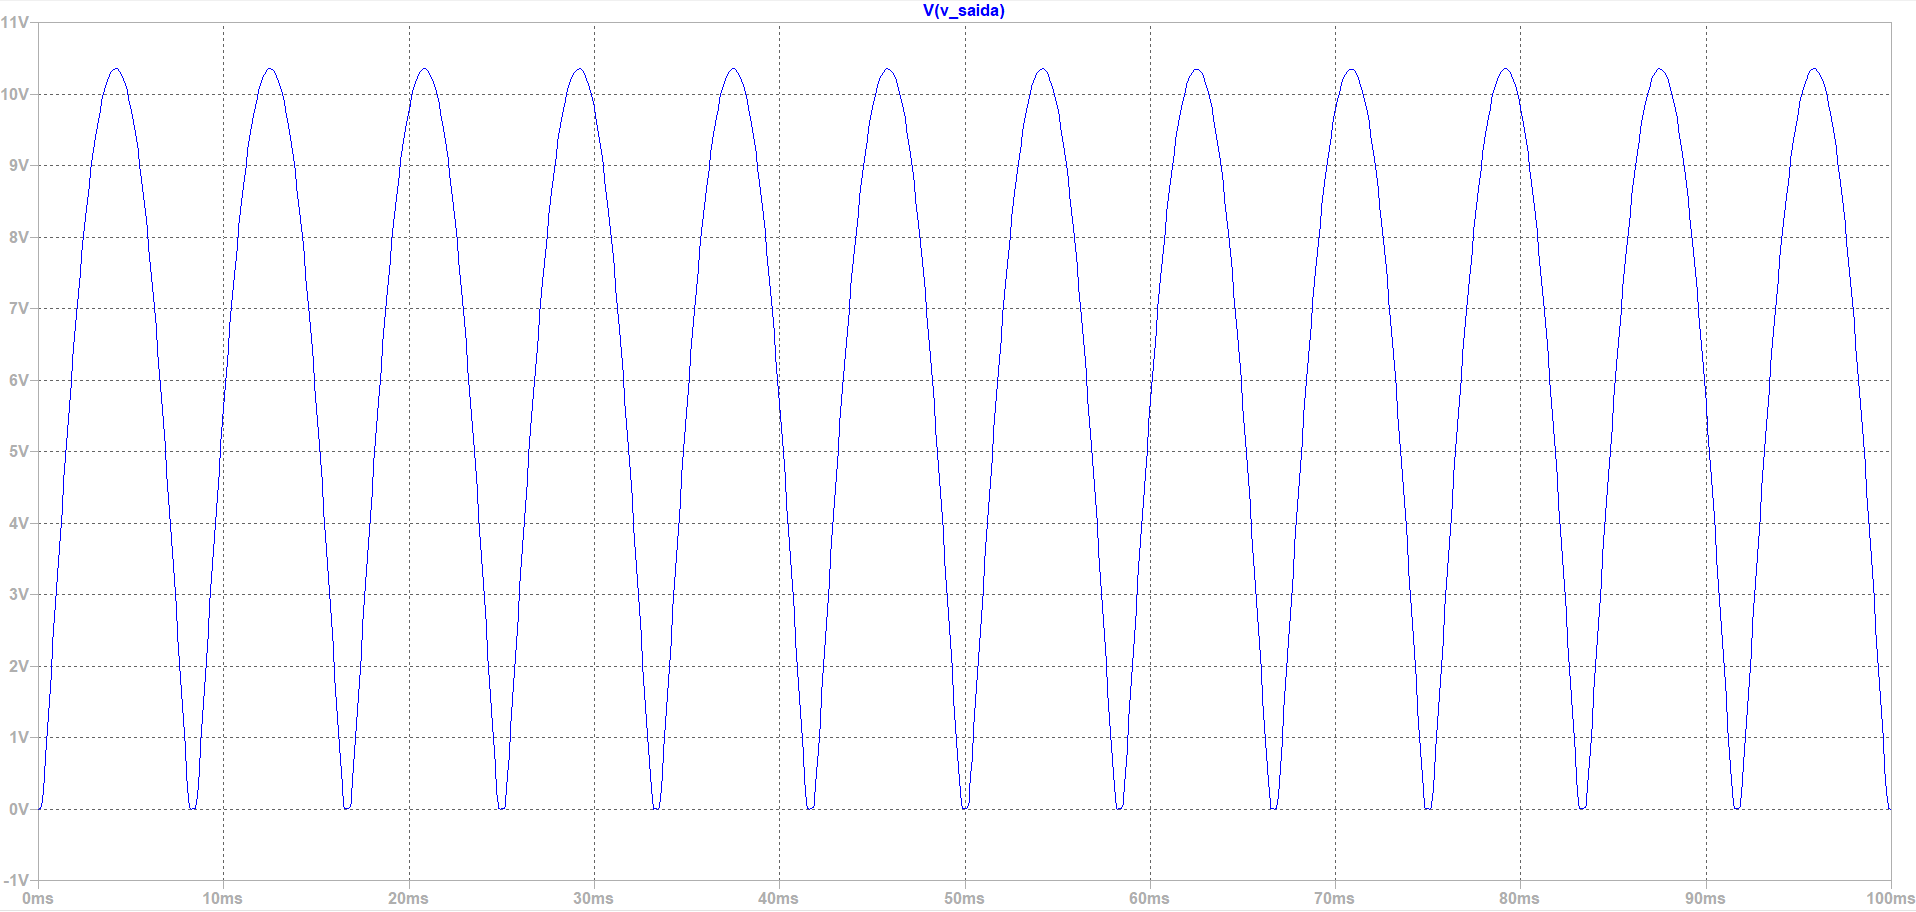
\includegraphics[width=\linewidth]{imgs/cardoso/resultados/simulacao_item_4_exp5.png}
        \vspace{2pt}
        {\small (d) Tensão: Onda completa sem filtro.}
    \end{minipage}
    
    \vspace{12pt}

    \begin{minipage}[b]{0.48\linewidth}
        \centering
        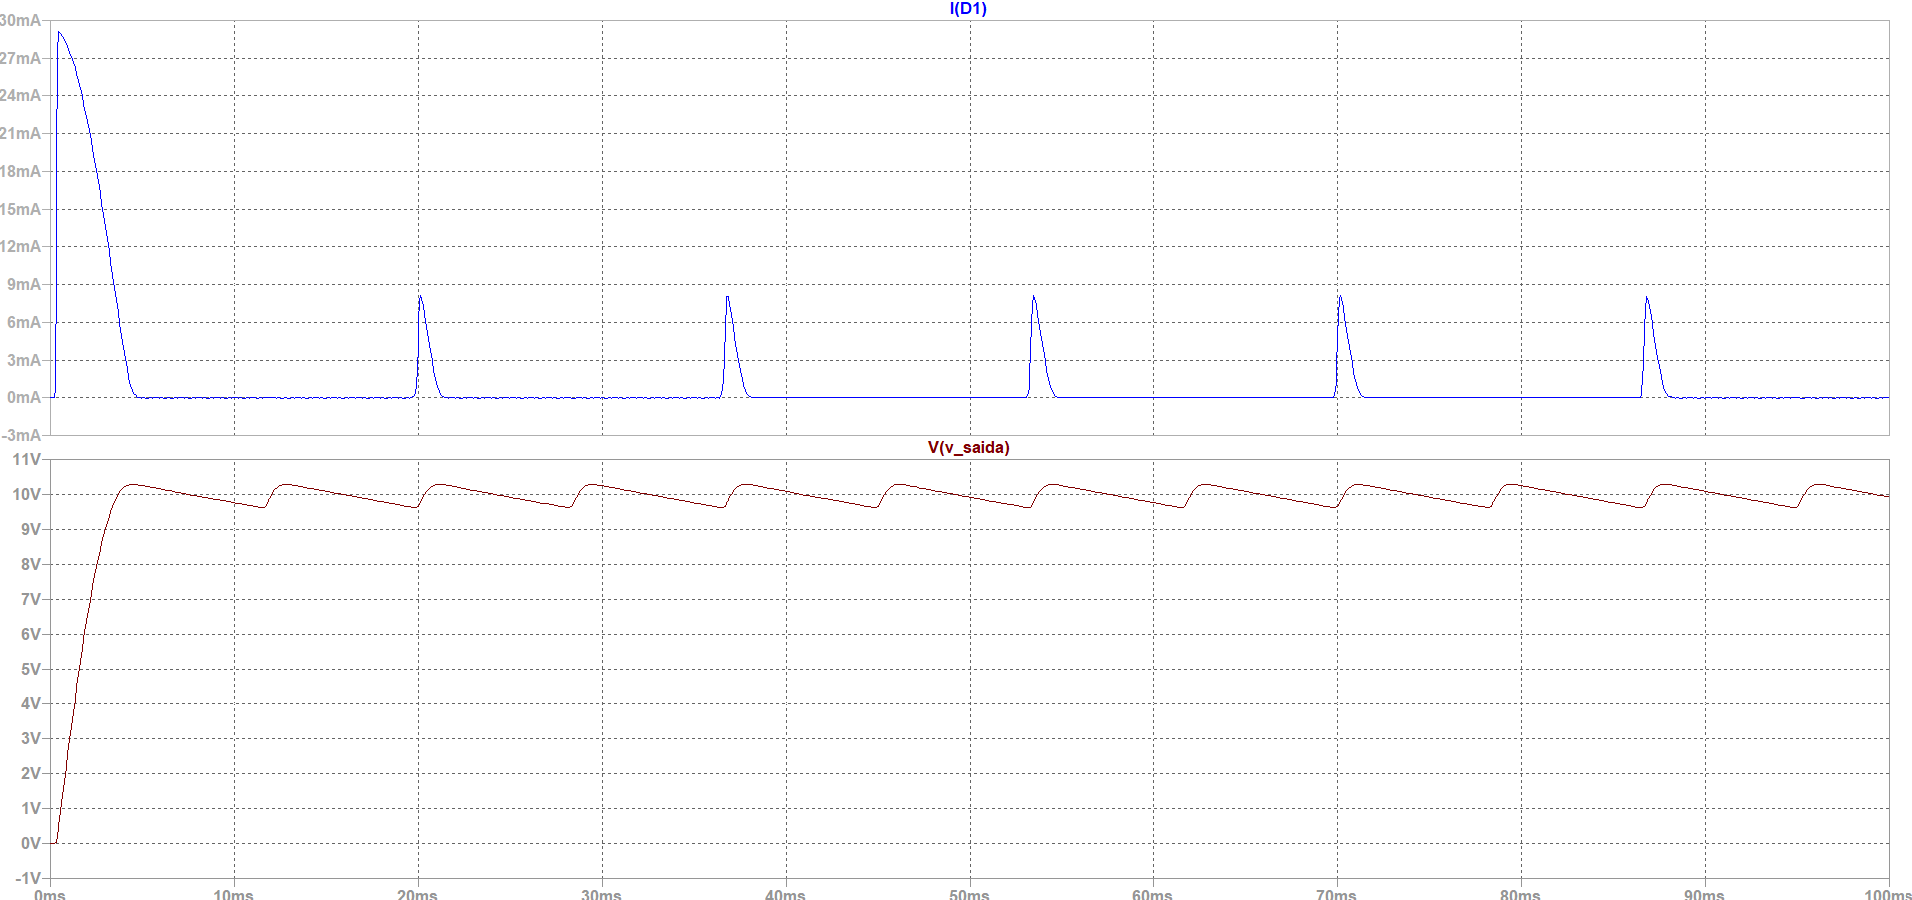
\includegraphics[width=\linewidth]{imgs/cardoso/resultados/simulacao_item_5_exp5.png}
        \vspace{2pt}
        {\small (e) Filtro na onda completa ($6{,}8\text{ }\mu\text{F}$).}
    \end{minipage}
    \hfill
    \begin{minipage}[b]{0.48\linewidth}
        \centering
        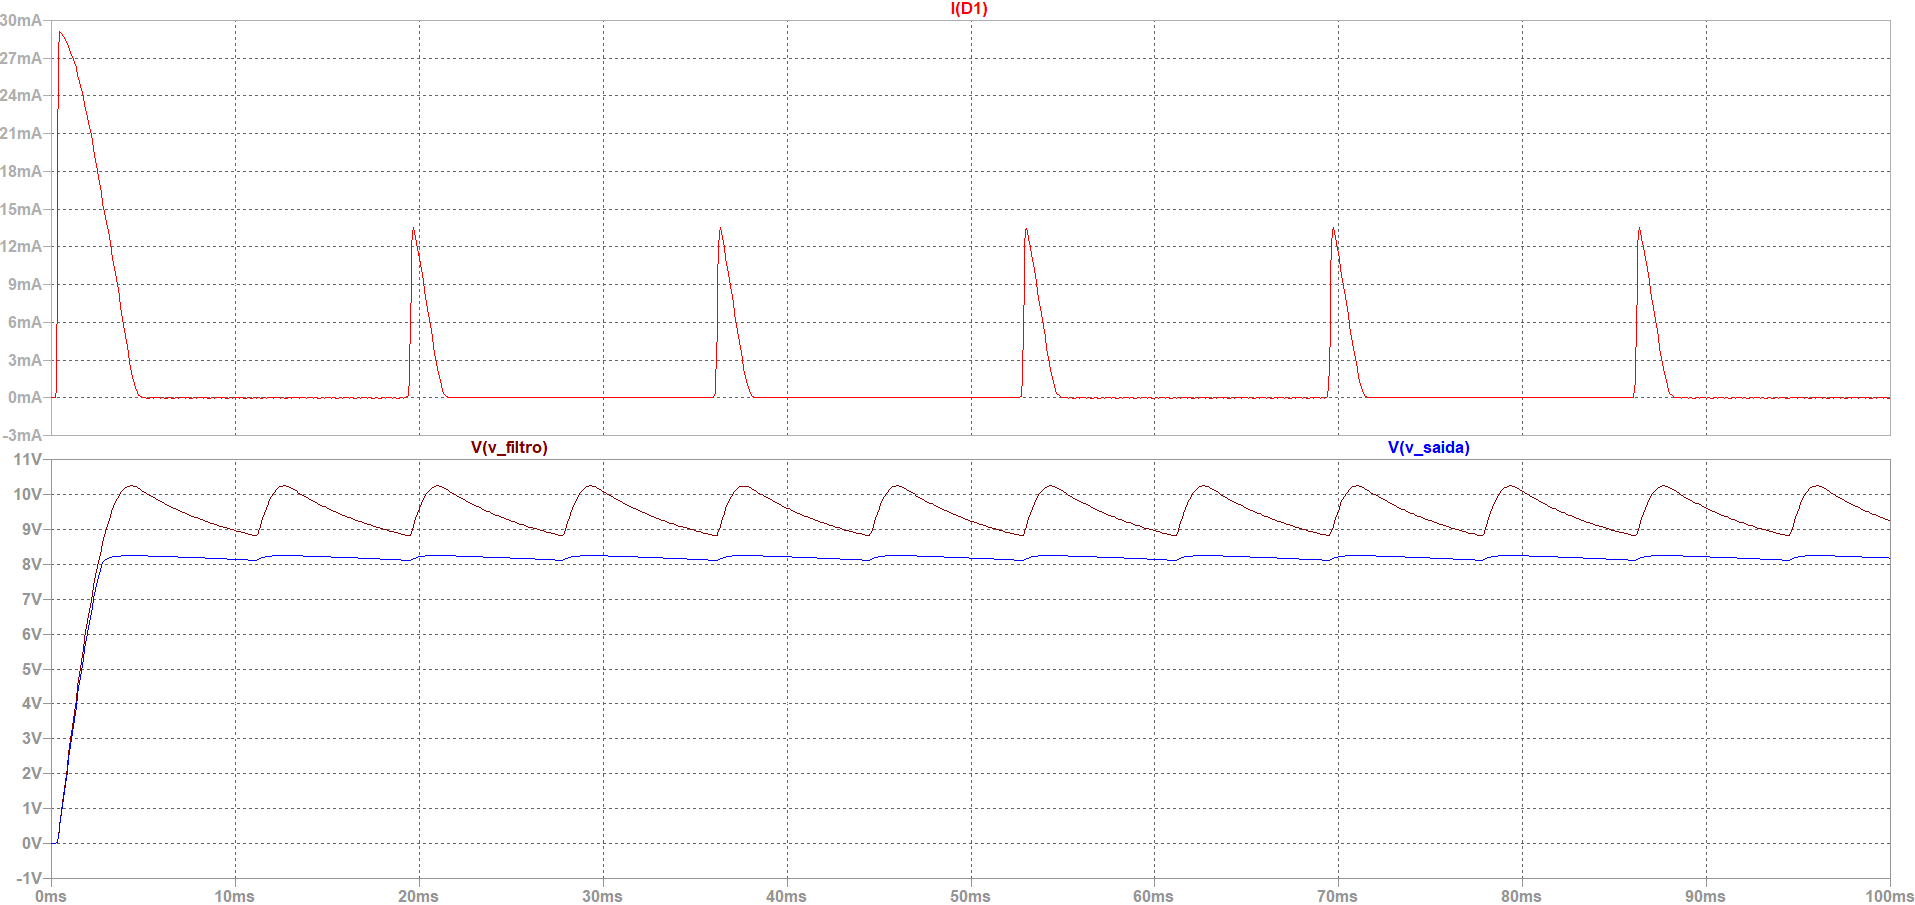
\includegraphics[width=\linewidth]{imgs/cardoso/resultados/simulacao_item_6_exp5.png}
        \vspace{2pt}
        {\small (f) Regulação final com Zener ($8{,}2\text{ V}$).}
    \end{minipage}
    \caption{Resultados gráficos das simulações de projeto dos estágios da fonte linear (matrícula 23/1038626).}
    \label{fig:graficos_cardoso}
\end{figure}

\subsection{Circuito montado}

% Para cada grandeza, o que o projeto do integrante montado previa, o que a simulação com os
% valores medidos devolveu, e o que vocês mediram na bancada. É desta tabela que sai a
% discussão.

% \begin{center}
% \begin{tabular}{@{}lrrrr@{}}
% \toprule
% \textbf{Grandeza} & \textbf{Projeto} & \textbf{Sim. montagem} & \textbf{Medido} &
% \textbf{Erro} \\
% \midrule
% & & & & \\
% \bottomrule
% \end{tabular}
% \end{center}

\section{Discussão}

% Percorra as três comparações na ordem em que aparecem no quadro da Seção~4: a conta contra
% a simulação de projeto, esta contra a simulação da montagem, e esta contra a medição. Cada
% passo isola uma causa, e a discussão fica bem mais curta quando eles não se misturam.

% Compare também os projetos dos integrantes entre si. Como as especificações são diferentes,
% os resultados diferem, e mostrar que essa diferença é a que a teoria previa vale mais do
% que repetir três vezes a mesma análise.

% Sempre que uma divergência for maior do que a incerteza esperada, aponte uma causa concreta
% e diga como ela poderia ser reduzida. Vale, por exemplo, a tolerância do componente, a
% resistência série do indutor, a impedância de entrada do osciloscópio, a banda do
% amplificador ou a resolução da varredura.

% Quando previsto e obtido coincidirem, explique por que era esperado que coincidissem, e o
% que essa coincidência não permite concluir.

% Por fim, retome as hipóteses que vocês declararam na fundamentação e diga quais se
% confirmaram. Se algo observado contrariar a previsão, resolva a contradição aqui.

\section{Conclusão}

% Retome o objetivo que vocês anunciaram na introdução e responda se ele foi atingido,
% apoiando a resposta em um número. Aponte a principal limitação do que foi feito e o que
% ela impede de afirmar. Evite trazer resultado novo nesta seção.

\section{Referências}

\begin{referencias}
\item SEDRA, A.~S.; SMITH, K.~C. \emph{Microeletrônica}. 5.~ed. São Paulo: Pearson
      Prentice Hall, 2007.
\item BOYLESTAD, R.~L.; NASHELSKY, L. \emph{Dispositivos Eletrônicos e Teoria de
      Circuitos}. 11.~ed. São Paulo: Pearson Education do Brasil, 2013.
\end{referencias}

\end{document}
